\documentclass[12pt]{elegantbook}

\definecolor{LightGray}{gray}{0.9}
\newcommand{\CN}{BIOS 7300\\[0.5cm] Survival Data Analysis}
\newcommand{\Ti}{Homework 5}
\newcommand{\Pf}{Dr. Tang}
\newcommand{\FN}{Zehao}
\newcommand{\LN}{Wang}
\usepackage[fontsize=14pt]{fontsize}

\usepackage{longtable}

\usepackage{minted}

\usepackage{enumitem}
\renewcommand{\chaptername}{Homework}
\begin{document} 
\begin{titlepage}
    \begin{center}    
    
\includegraphics[width=0.6\textwidth]{Tulane.png}\\[1cm]    
    
    \textsc{\Huge \CN}\\[0.5cm]
    \textsc{\large \Pf}\\[1.0cm]
    
    \textsc{\LARGE \Ti}\\[0.5cm]
    \textsc{\large \LN, \FN}\\
    {Master student in Statistics of Math Dept.}
    
    % Author and supervisor
    
    \vfill
    
    % Bottom of the page
    {\Large \emph{\today}}
    
    \end{center}
\end{titlepage}

\thispagestyle{empty}
\tableofcontents
\setcounter{chapter}{4}
\chapter{}

    
    \begin{exercise*}[1]
        In a study of smoking (SAS dataset “smoke”), there were two treatments (patch only and combination). Ignoring other covariates, we may apply log-rank test to compare the two treatment groups. Alternatively, we may fit a proportional hazards model with the treatment as the only predictor and test if it is significantly associated with the survival outcome. 
        \begin{enumerate}[(a)]
            \item Perform the log-rank test to check the treatment effect. 
            \item Fit a proportional hazards model to assess the treatment effect.
            \item Compare (a) and (b). When would you expect to have the same statistics and p-values for tests in parts (a) and (b). 
        \end{enumerate}
    \end{exercise*}

    \begin{solution}
        \begin{enumerate}[(a)]
            \item \begin{minted}[frame=lines,
                framesep=2mm,
                baselinestretch=1.2,
                bgcolor=LightGray,
                fontsize=\footnotesize]{SAS}
DATA HW5_1; 
SET "Z:\Documents\GitHub\MS-Stat-Tulane
\Survival Data Analysis\HW05\smoke.sas7bdat"; 
PROC LIFETEST DATA = HW5_1 METHOD = KM; 
TIME time*status(0); 
STRATA treat; 
RUN; 
            \end{minted}
            \begin{figure}[H]
                \centering
                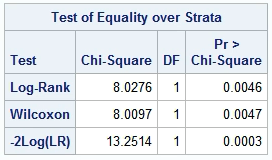
\includegraphics[width=.25\textwidth]{HW5_1_1.png}
            \end{figure}
            From the test, we can see that the p-value is $0.0046<0.05$. So, we can reject the null hypothesis and get that the treatment effect is significant. 
            \item \begin{minted}[frame=lines,
                framesep=2mm,
                baselinestretch=1.2,
                bgcolor=LightGray,
                fontsize=\footnotesize]{SAS}
PROC PHREG DATA = HW5_1;
CLASS treat;
MODEL time*status(0) = treat;
HAZARDRATIO treat / AT () DIFF=ALL;
RUN;
            \end{minted}
            \begin{figure}[H]
                \centering
                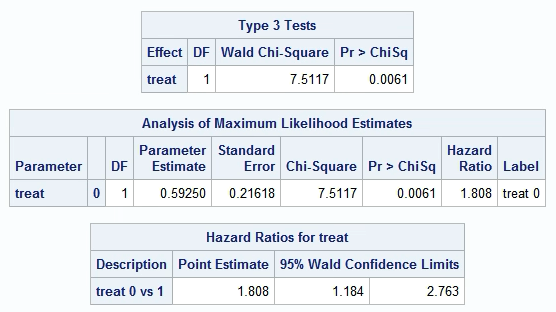
\includegraphics[width=.6\textwidth]{HW5_1_2.png}
            \end{figure}
            From the hazard model, treatment effect is significant, too. 
            \item If the hazard function has no difference, the statistics and p-values should be the same.
        \end{enumerate}
    \end{solution}

    \begin{exercise*}[2]
        Use the data “Survival of liver transplant recipients.dat”, with disease and cof as predictors. We treat both of them as factors and also consider their interaction. So the model is “survival time$\sim$disease | cof”. Based on the model,
        \begin{enumerate}[(a)]
            \item Estimate the hazard ratio between the group with disease = 1 and disease =3, both with cof=4; 
            \item Estimate the hazard ratio between the group with disease=1 and cof=0 and the group with disease=3 and cof=4. 
            \item Is the interaction between the disease and cof significant?
        \end{enumerate}
    \end{exercise*}

    \begin{solution}
        \begin{enumerate}[(a)]
            \item \begin{minted}[frame=lines,
                framesep=2mm,
                baselinestretch=1.2,
                bgcolor=LightGray,
                fontsize=\footnotesize]{SAS}
DATA HW5_2; 
INFILE "Z:\Documents\GitHub\MS-Stat-Tulane
\Survival Data Analysis\HW05
\Survival of liver transplant recipients.dat" FIRSTOBS=2; 
INPUT patient age gender disease time status cof;
PROC PHREG DATA = HW5_2;
CLASS disease (ref=first) cof (ref="0");
MODEL time*status(0) = disease | cof;
HAZARDRATIO disease / AT (cof = "4") DIFF=ALL;
RUN;
            \end{minted}
            \begin{figure}[H]
                \centering
                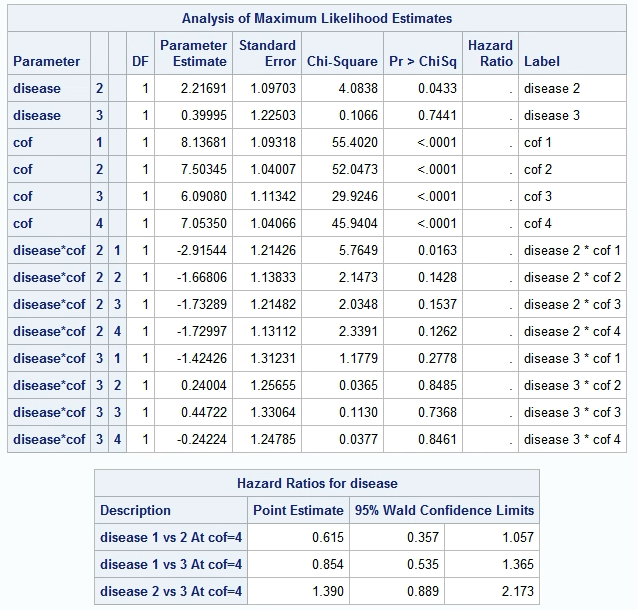
\includegraphics[width=.6\textwidth]{HW5_2_1.png}
            \end{figure}
            It is $0.854$. 
            \item HR at $disease=1$, $cof=0$ V.S. $disease=3$, $cof=4$ is: 
            \[
                \frac{h_0(t)}{HR(disease=3,\ cof=4)}=\exp(-0.40-7.054+0.242)=7.377\times10^{-4}. 
            \]
            \item \begin{figure}[H]
                \centering
                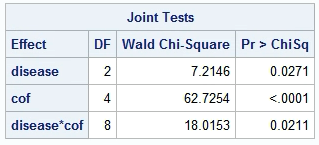
\includegraphics[width=.35\textwidth]{HW5_2_2.png}
            \end{figure}
            p-value is $0.0211<0.05$. So, the interaction is significant.
        \end{enumerate}
    \end{solution}

    \begin{exercise*}[3]
        A Cox proportional hazards model with a single factor predictor (Group with levels 1, 2, 3, and 4) is applied to a survival data. The parameter estimates are given the following table: 
        \begin{figure}[H]
            \centering
            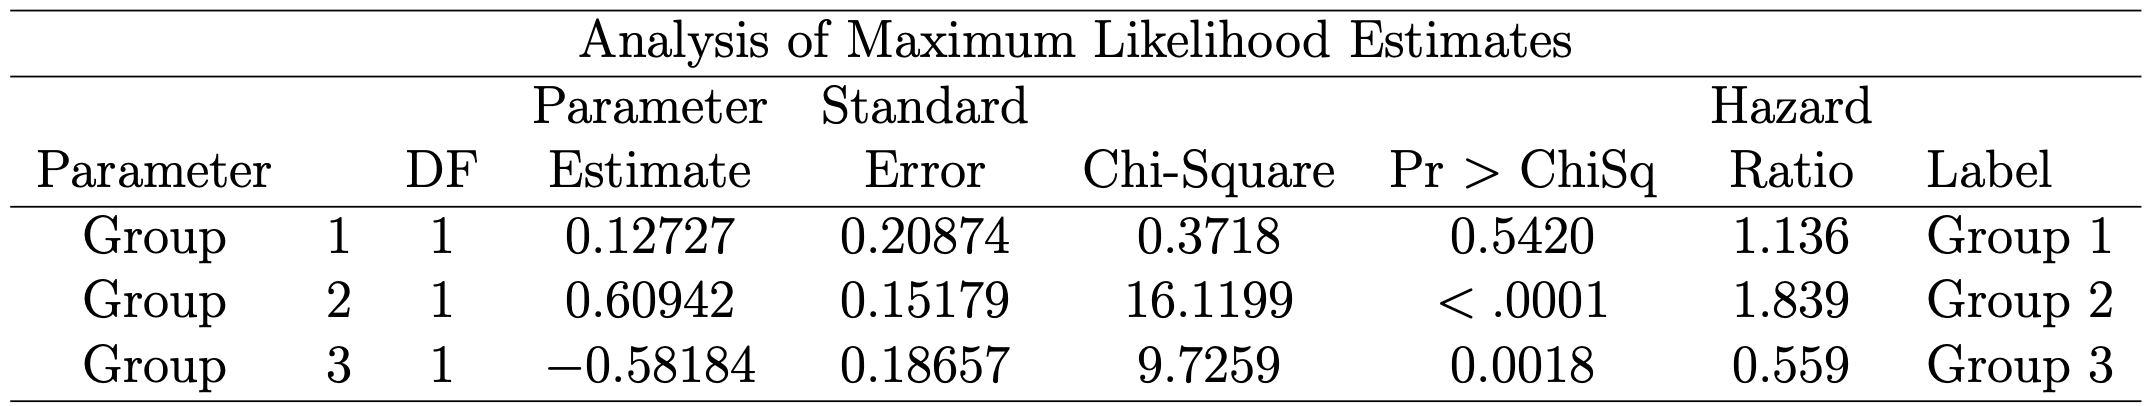
\includegraphics[width=.95\textwidth]{h5_q3_1.png}
        \end{figure}
        The baseline survival function estimate (estimate for Group 4) is given in the table. For example, $\hat{S}(70)=0.70822$ for the reference group. 
        \begin{enumerate}[(a)]
            \item Estimate $\hat{S}(70)$ for the other three groups. 
            \item Estimate the median survival times of the four groups. 
        \end{enumerate}
        {\footnotesize
    \begin{longtable}[c]{lll|lll|lll|lll}
    \hline
    
    Obs & time & Survival & Obs & time & Survival & Obs & time & Survival & Obs & time & Survival \\ \hline
    \endfirsthead
    %
    \endhead
    %
    \hline
    \endfoot
    %
    \endlastfoot
    %
    
    1   & 0    & 1        & 55  & 92   & 0.67366  & 109 & 598  & 0.44555  & 163 & 1633 & 0.21459  \\
    2   & 0    & 0.9935   & 56  & 96   & 0.66978  & 110 & 601  & 0.44149  & 164 & 1659 & 0.21035  \\
    3   & 1    & 0.99024  & 57  & 99   & 0.6659   & 111 & 614  & 0.43744  & 165 & 1755 & 0.20611  \\
    4   & 2    & 0.97407  & 58  & 110  & 0.66202  & 112 & 617  & 0.43338  & 166 & 1836 & 0.2019   \\
    5   & 3    & 0.96425  & 59  & 115  & 0.65815  & 113 & 641  & 0.42929  & 167 & 1901 & 0.19773  \\
    6   & 4    & 0.9544   & 60  & 116  & 0.65427  & 114 & 642  & 0.42522  & 168 & 1947 & 0.1936   \\
    7   & 5    & 0.94777  & 61  & 117  & 0.65039  & 115 & 654  & 0.42112  & 169 & 1983 & 0.18946  \\
    8   & 6    & 0.94443  & 62  & 121  & 0.64651  & 116 & 704  & 0.41704  & 170 & 1990 & 0.18532  \\
    9   & 8    & 0.93113  & 63  & 122  & 0.64261  & 117 & 727  & 0.41297  & 171 & 2039 & 0.18116  \\
    10  & 9    & 0.92104  & 64  & 125  & 0.63871  & 118 & 767  & 0.4089   & 172 & 2043 & 0.17699  \\
    11  & 10   & 0.91428  & 65  & 128  & 0.63481  & 119 & 780  & 0.40483  & 173 & 2044 & 0.17287  \\
    12  & 12   & 0.90072  & 66  & 131  & 0.63091  & 120 & 795  & 0.39667  & 174 & 2050 & 0.16875  \\
    13  & 13   & 0.89043  & 67  & 133  & 0.62314  & 121 & 806  & 0.39258  & 175 & 2089 & 0.16467  \\
    14  & 14   & 0.88695  & 68  & 140  & 0.61529  & 122 & 810  & 0.3885   & 176 & 2111 & 0.16063  \\
    15  & 15   & 0.88002  & 69  & 143  & 0.61134  & 123 & 822  & 0.38437  & 177 & 2113 & 0.15659  \\
    16  & 17   & 0.87305  & 70  & 157  & 0.60738  & 124 & 874  & 0.38025  & 178 & 2193 & 0.1525   \\
    17  & 18   & 0.86607  & 71  & 165  & 0.60341  & 125 & 894  & 0.3761   & 179 & 2272 & 0.1484   \\
    18  & 19   & 0.86256  & 72  & 174  & 0.59945  & 126 & 912  & 0.37197  & 180 & 2300 & 0.14436  \\
    19  & 20   & 0.85202  & 73  & 176  & 0.59548  & 127 & 915  & 0.36786  & 181 & 2303 & 0.14031  \\
    20  & 21   & 0.84145  & 74  & 180  & 0.59151  & 128 & 918  & 0.36375  & 182 & 2316 & 0.13626  \\
    21  & 22   & 0.83434  & 75  & 185  & 0.58756  & 129 & 935  & 0.35965  & 183 & 2348 & 0.13211  \\
    22  & 23   & 0.83076  & 76  & 199  & 0.58358  & 130 & 957  & 0.35556  & 184 & 2400 & 0.12796  \\
    23  & 25   & 0.82004  & 77  & 201  & 0.5796   & 131 & 965  & 0.35147  & 185 & 2460 & 0.12381  \\
    24  & 26   & 0.81644  & 78  & 219  & 0.57562  & 132 & 988  & 0.34734  & 186 & 2463 & 0.11966  \\
    25  & 27   & 0.81282  & 79  & 229  & 0.57164  & 133 & 1043 & 0.34323  & 187 & 2538 & 0.11552  \\
    26  & 28   & 0.80558  & 80  & 230  & 0.56765  & 134 & 1047 & 0.33912  & 188 & 2559 & 0.11124  \\
    27  & 29   & 0.80195  & 81  & 236  & 0.56367  & 135 & 1104 & 0.33501  & 189 & 2602 & 0.10696  \\
    28  & 31   & 0.79832  & 82  & 241  & 0.55969  & 136 & 1112 & 0.3309   & 190 & 2619 & 0.10275  \\
    29  & 34   & 0.79105  & 83  & 247  & 0.5557   & 137 & 1114 & 0.32678  & 191 & 2669 & 0.09862  \\
    30  & 35   & 0.78739  & 84  & 249  & 0.55172  & 138 & 1120 & 0.32267  & 192 & 2685 & 0.09457  \\
    31  & 38   & 0.78372  & 85  & 255  & 0.54771  & 139 & 1129 & 0.3185   & 193 & 2693 & 0.09051  \\
    32  & 40   & 0.78003  & 86  & 271  & 0.54367  & 140 & 1151 & 0.31437  & 194 & 2848 & 0.08654  \\
    33  & 41   & 0.77265  & 87  & 277  & 0.53963  & 141 & 1152 & 0.31023  & 195 & 2864 & 0.08256  \\
    34  & 42   & 0.76892  & 88  & 292  & 0.53556  & 142 & 1207 & 0.30206  & 196 & 2892 & 0.07867  \\
    35  & 45   & 0.76517  & 89  & 294  & 0.53151  & 143 & 1208 & 0.2979   & 197 & 2948 & 0.07486  \\
    36  & 46   & 0.76141  & 90  & 299  & 0.52745  & 144 & 1214 & 0.29373  & 198 & 2962 & 0.07102  \\
    37  & 51   & 0.7539   & 91  & 305  & 0.5234   & 145 & 1232 & 0.2896   & 199 & 2972 & 0.06727  \\
    38  & 52   & 0.75012  & 92  & 324  & 0.51931  & 146 & 1240 & 0.28545  & 200 & 2981 & 0.06362  \\
    39  & 53   & 0.74259  & 93  & 337  & 0.51523  & 147 & 1311 & 0.28131  & 201 & 3103 & 0.05996  \\
    40  & 57   & 0.73879  & 94  & 352  & 0.51114  & 148 & 1320 & 0.27717  & 202 & 3162 & 0.0563   \\
    41  & 58   & 0.73498  & 95  & 370  & 0.50706  & 149 & 1339 & 0.27297  & 203 & 3185 & 0.05243  \\
    42  & 59   & 0.73117  & 96  & 373  & 0.50296  & 150 & 1392 & 0.2688   & 204 & 3192 & 0.04857  \\
    43  & 60   & 0.72736  & 97  & 386  & 0.49887  & 151 & 1415 & 0.26463  & 205 & 3259 & 0.0447   \\
    44  & 63   & 0.72355  & 98  & 392  & 0.49477  & 152 & 1420 & 0.26046  & 206 & 3289 & 0.04097  \\
    45  & 64   & 0.71972  & 99  & 427  & 0.49067  & 153 & 1436 & 0.25632  & 207 & 3346 & 0.03739  \\
    46  & 65   & 0.71588  & 100 & 496  & 0.48658  & 154 & 1437 & 0.25219  & 208 & 3357 & 0.03381  \\
    47  & 68   & 0.71205  & 101 & 508  & 0.48245  & 155 & 1456 & 0.24805  & 209 & 3534 & 0.03023  \\
    48  & 69   & 0.70822  & 102 & 509  & 0.47832  & 156 & 1458 & 0.24391  & 210 & 3575 & 0.02665  \\
    49  & 74   & 0.70057  & 103 & 540  & 0.47421  & 157 & 1529 & 0.23977  & 211 & 3745 & 0.02307  \\
    50  & 80   & 0.69674  & 104 & 546  & 0.47009  & 158 & 1535 & 0.23563  & 212 & 3764 & 0.01807  \\
    51  & 84   & 0.6929   & 105 & 549  & 0.46598  & 159 & 1558 & 0.23149  & 213 & 3775 & 0.01288  \\
    52  & 85   & 0.68907  & 106 & 559  & 0.46186  & 160 & 1577 & 0.22735  & 214 & 4083 & 0.00527  \\
    53  & 87   & 0.68138  & 107 & 591  & 0.4537   & 161 & 1614 & 0.22315  & 215 & 4215 & 0.00088  \\
    54  & 88   & 0.67752  & 108 & 593  & 0.44962  & 162 & 1628 & 0.21888  &     &      &          \\ \hline
    \end{longtable}
    }
    \end{exercise*}

    \begin{solution}
        \begin{enumerate}[(a)]
            \item $h_0(t)=0.70822$. So, 
            \[\hat{S}_1(70)=0.70822^{\exp(0.12727)}=0.6758. \]
            \[\hat{S}_2(70)=0.70822^{\exp(0.60942)}=0.5301. \]
            \[\hat{S}_3(70)=0.70822^{\exp(-0.58184)}=0.8246. \]
            \item For Group 4: $t=386$. 
            
            For Group 1: \[S_4(t)=e^{\exp(-0.12727)\log 0.5}\Rightarrow t=277. \]

            For Group 2: \[S_4(t)=e^{\exp(-0.60942)\log 0.5}\Rightarrow t=87. \]

            For Group 3: \[S_4(t)=e^{\exp(0.58184)\log 0.5}\Rightarrow t=1240. \]
        \end{enumerate}
    \end{solution}
    
\end{document}